In this chapter, we perform various experiments to get a better understanding of the IRS kernel space implementations proposed in the previous chapter. 
The experiments are intended to provide a comparison between user space and kernel space IRS implementations. 
The comparison between the above implementations are evaluated across multiple processor cores ranging from two to eight cores.  
We evaluate kernel space solutions based on the number of calls made to kernel space for synchronization. 
Four benchmarking programs are used for all the above mentioned evaluations.

\section{Setup}

The evaluation is performed with a virtual machine running on a hardware with Intel Xeon E5-2650 - 2.00 GHz(16 cores) configured with Ubuntu 17.04 as the operating system. 
It is configured with 4GB RAM and 80GB hard disk. 
The virtual machine(VM) is configured with the LLVM-CLANG 3.9, GCC 4.9 and Boost 1.6.2. 
We use multiple VM configurations ranging from two cores to eight cores for various evaluations. 
Configurations by scaling the number of processor cores is mainly intended to perform a scaled evaluation of cores to number of threads across various IRS implementations for a given benchmark.

\section*{Note}

We would be using the following abbreviations in the rest of the evaluations for simplicity of expression.
\begin{itemize}
\item {IRS\_Sh} - One of the IRS user space implementation discussed in sections~\ref{iter_rel_sched} and \ref{mot}. 
It addresses the use of a busy waiting design for blocking a thread and use the other threads in the thread pool to signal the blocked thread. 
Thus, making the scheduling decision shared among the threads. 
This design does not have an additional thread for handling the scheduling decisions. 
\item {IRS\_Opt} - Another user space IRS solution discussed in sections~ \ref{iter_rel_sched} and \ref{mot}. 
It uses an additional thread for handling the scheduling decisions and uses conditional variables to block a certain thread when memory access is restricted. 
\item {Proto\_1} - Section~\ref{sync_des} highlights all the prototypes used in this thesis to provide various solutions addressing the transition of scheduling decision to kernel space. 
Prototype 1 is the first synchronization discussed in section~\ref{sync_des} which uses a shared scheduler design similar to IRS\_Sh but, the blocking of threads is enforced by using semaphores in kernel space. 
\item {Proto\_2} - Prototype 2 is an extension of the previous prototype. 
Prototype also uses semaphores in kernel space for blocking a given thread but, the signaling the blocked thread is done by an additional thread which is similar to IRS\_Opt.
\item {Proto\_3} - Prototype 3 is a lot similar to Prototype 1 in the nature of behavior when it comes to design and its approach to scheduling. 
Main difference of Prototype 3 compared to Prototype 1 is the use of scheduler APIs instead of semaphores for blocking a given thread. 
\item {Proto\_4} - Prototype 4 is a design variant of Prototype 2. It uses the same scheduling approach as Prototype 2 but, differs in the blocking of a given thread. 
It uses scheduler APIs instead of semaphores. 
\item {Proto\_5} - Prototype 5 are an extension of Prototype 2, it is one of the designs which addresses the second approach discussed in section~\ref{sec_app}. 
As discussed in section~\ref{sec_app} it uses a proxy checking of memory access permission in user space.
\item {Proto\_6} - Prototype 6 are an extension of Prototype 4, it is another design which addresses the second approach discussed in section~\ref{sec_app}. 
As discussed in section~\ref{sec_app} it uses a proxy checking of memory access permission in user space.

\end{itemize}

In short, Proto\_1, Proto\_2, Proto\_3, Proto\_4 use the first approach discussed in section~\ref{fir_app}. 
Whereas, Proto\_5 and Proto\_6 use the second approach discussed in section~\ref{sec_app}.

\section{Benchmarks}

We use four different benchmarking programs for the evaluation of this thesis. 
The bench-marking programs are:
\begin{itemize}
\item{Fibonacci} - Program runs with two threads computing the Fibonacci numbers for 25 iterations per thread.
\item{Last Zero} - \citet{abdulla2014optimal} presents this benchmark for evaluating their work. The benchmark program runs with 16 threads.
\item{Indexer}- \citet{dynamic_por} use this benchmark program for evaluation of their work. The benchmark program runs with 15 threads.
\item{Dining Philosophers Problem} - The benchmark program runs with 16 threads. 
This benchmark is motivated from the solution presented in \citet{silberschatz2014operating}.
\end{itemize}

We generate memory constraints(constraints addressing shared memory events) for the above benchmarks in the form of an execution trace stored in a trace file. 
The trace file is a graphviz representation. 
The trace file is manually generated based on the benchmark in use. 
It could be automated in the future by having an automated verifier as discussed in the section~\ref{theor_des}.
The graphviz representation is converted manually into a vector clock representation containing only the shared memory dependencies between the  threads. 
The vector clock representation is a string depicting the inter-dependencies between threads on a shared memory event. 
We use the vector clock representation for the prototypes and graphviz file for the user space IRS solutions. 
Both the representations are logically equivalent. 
More details about their representation and conversion can be found in appendix C. 

\section{Evaluation Metrics}

\subsection{Execution Overhead}

Evaluation is done between the IRS user space solutions vs kernel space solutions. 
Execution overhead is calculated for each solution with respect to the plain execution of the benchmarking program. 
Unconstrained execution of the program is considered as plain execution. 

$$Execution Overhead = (T_{constr} - T_{plain})/T_{plain} * 100$$

$T_{constr}$ is the execution time of the bench-marking program when executed with scheduling constraints. 
$T_{plain}$ is the plain execution time of the same bench-marking program. 
We expect to monitor the performance of various IRS implementations by checking this metric. 
If execution overhead for a certain IRS design is the smallest, that design is considered to give the best performance. 

\subsection{Number of necessary synchronization calls} 

This metric used to realize the number of necessary calls made to the kernel space for synchronization purposes. 
The number of synchronization calls are primarily the number of IOCTL calls made under the commands: context\_switch, signal\_all\_other\_threads or set\_clock. 
The term `necessary' is validated based on the number of IOCTL calls which actually performs the synchronization operations for the commands mentioned above. 
Whereas in case of `unnecessary' calls, we observe a behavior of IOCTL calls returned to the user space without any major influence or changes in the kernel space. 
We record the number of IOCTL calls with the command context\_switch and determine the prototypes which provide a smaller overhead. 
We expect some of the prototypes to make unnecessary calls to kernel space when requesting a context switch. 
These unnecessary calls are expected to generate more overhead on execution time. 
For multithreaded programs which have extremely less number of memory constraints compared to the total number of shared memory events is expected to yield poor performance on the prototypes which yield unnecessary calls. 
Thus, making this evaluation metric a crucial parameter when comparing various prototypes. 
More explanation about such a behavior is discussed in section~\ref{sec_app}.  
We describe the use of this metric more in this section~\ref{vol_kernel_calls}.  


\section{Number of synchronization calls \label{vol_kernel_calls}}

We evaluate the number of necessary calls made to kernel space for synchronization operation. 
The evaluation is done across all six prototypes described in this thesis. 
The benchmark used for the evaluation is Fibonacci. 
The Fibonacci benchmark presents different levels of memory constraints via its traces. 
It has three traces providing 98 constraints, 44 constraints and 24 constraints respectively. 

\begin{table}[h]
\begin{center}
 \begin{tabular}{|c c c|} 
 \hline
 & Prototype 1-4 & Prototype 5-6\\ %[0.5ex] 
 \hline
 Trace-1 & 300 & 175\\ 
 Trace-2 & 300 & 150\\
 Trace-3 & 300 & 150\\
 \hline
\end{tabular}
\end{center}
\caption{Number of IOCTL calls}
\label{num_ioctls}
\end{table}
\begin{table}
\begin{center}
 \begin{tabular}{|c c c|} 
 \hline
 & Prototype 1-4 & Prototype 5-6\\ %[0.5ex] 
 \hline
 Trace-1 & 150 & 27\\ 
 Trace-2 & 150 & 0\\
 Trace-3 & 150 & 0\\
 \hline
\end{tabular}
\end{center}
\caption{Number of context switch calls}
\label{num_ctxts}
\end{table}

From the tables~\ref{num_ioctls} and \ref{num_ctxts}, it is evident that prototypes 5 and 6 reduce the number of calls made to kernel space. 
Prototypes 5 \& 6 are expected to provide better performance compared to other prototypes, when the number of memory constraints in the trace is extremely less than the total number of shared memory events in the benchmark as depicted in equation~\ref{mem_cond}. 
Section~\ref{sec_app} provides a detailed explanation of the approach used in prototypes 5 and 6, and the reason for their better performance. 

The Fibonacci benchmark has two threads with a total of 75 shared-memory events per thread. 
Thus, making a total of 150 memory events. 
For every shared-memory event, prototypes 1-4 trigger IOCTL calls to kernel space for context\_switch, signal\_all\_other\_threads or set\_clock. 
Therefore, having a total number of IOCTL calls as 300. 
In case of prototype 5-6, we have a proxy checking for shared memory access  in user space which drastically reduces the calls to kernel space for additional synchronization. 
The set\_clock ioctl command is the only call made consistently for every memory access when using prototypes 5-6.

\begin{table}[h]
\begin{center}
 \begin{tabular}{|c c c c c c c|} 
 \hline
 & Proto-1 & Proto-2 & Proto-3 & Proto-4 & Proto-5 & Proto-6\\ %[0.5ex] 
 \hline
 Trace-1 & 406.833 & 454.785 & 385.416 & 455.745 & $277.793$ & $275.343$ \\ 
 Trace-2 & 367.199 & 520.352 & 352.506 & 509.843 & $160.266$ & $160.307$ \\
 Trace-3 & 351.029 & 416.653 & 333.704 & 412.206 & $152.425$ & $153.06$\\
 \hline
\end{tabular}
\end{center}
\caption{Execution overhead(\%) when compared with plain execution of Fibonacci across six prototypes}
\label{fib_exec_over}
\end{table}

Table~\ref{fib_exec_over} shows us that the execution overhead is drastically reduced for the prototypes 5 and 6. 
Reduction in the number of IOCTL calls is reason for such a difference in the execution overhead. 
Prototypes 5-6 provide lower execution time overhead compared to other prototypes, when the condition indicated in equation~\ref{mem_cond} is satisfied. 

\section{Comparison between user space and kernel space IRS solutions}

In this evaluation, we understand the merits and demerits in the performance of the six prototypes and the two user space IRS implementations. 
For this evaluation, we use four bench-marking programs - Fibonacci, Last Zero, Indexer and Dining Philosophers Problem. 
We scale the processor configuration from two to eight processor cores and monitor the changes in the performance overhead across the benchmarks - Last Zero, Indexer and Dining Philosophers Problem for the various IRS implementations. 
Fibonacci benchmark is evaluated only with the configuration of two processor cores because the number of threads configured for the benchmark is two. 
The best prototype among the six prototypes is chosen and compared with IRS user space implementation for each benchmark.
Scaling the number of cores aids in the scalability evaluation of various IRS implementations. 
Such an evaluation also helps to realize the possibility of false sharing problem in the designs. 

\subsection{Fibonacci}

\begin{figure}[h]
     \centering
     \subfloat[][User space vs Best Prototype]{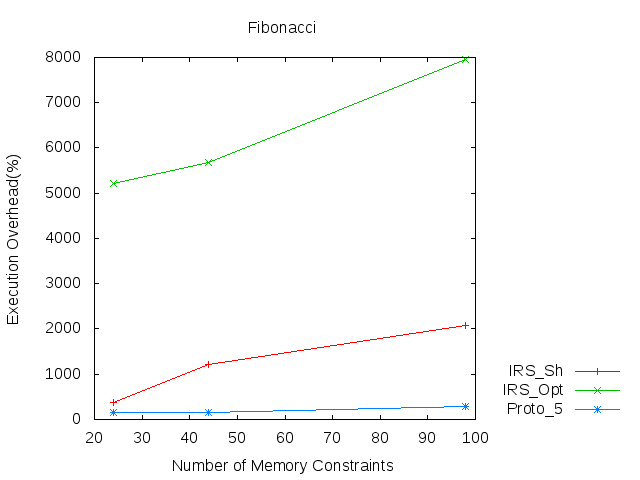
\includegraphics[scale=0.5]{../../evaluations/cores_2/eval_fibonacci_best.png}\label{fibonacci_best_cores_2}}
     \subfloat[][Comparison between prototypes]{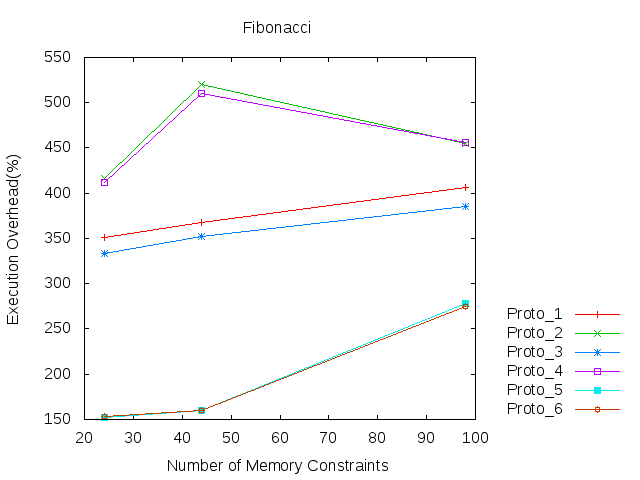
\includegraphics[scale=0.5]
{../../evaluations/cores_2/eval_fibonacci_protos.png}
\label{fibonacci_protos_cores_2}}
     \caption{Comparison of IRS with Fibonacci on two cores}
\end{figure}

Fibonacci benchmark has two threads at its disposal. 
The pseudo code of this benchmark is depicted in listing~\ref{code_fibonacci}. 
The trace files for this benchmark provides 98, 44 and 24 memory constraints. 
The memory constraints indicated in this benchmark are the shared memory dependencies between the two threads in the benchmark. 
The benchmark is configured to run for 25 iterations. 
For every iteration as seen in listing~\ref{code_fibonacci}, we have three shared memory event. 
These memory events include two consecutive reads and one final write. 
There are three memory events for iteration and there are two threads in total for this benchmark. 
Thus, having a total of 150 shared memory events. 
The execution overhead is expected to be higher when the number of memory constraints are close to total shared memory events. 
For the first trace file (98 memory constraints), we expect to have a higher execution overhead in IRS user space implementations and comparatively lower overhead in kernel space implementations. 
With the third trace(24 memory constraints), we expect the difference in the execution overhead of IRS user space solutions to the prototypes to be smaller. 
The key reason for such a behavior is that we expect the user space solutions to perform better when the number of memory constraints in the benchmarking programs are far less to the total number of shared memory events in the program. 

From figure~\ref{fibonacci_protos_cores_2}, we observe that Proto\_5 and Proto\_6 provide the best performance among all the prototypes. 
The reason for such a behavior is the condition depicted in equation~\ref{mem_cond} satisfies. 
Section~\ref{sec_app} presents a detailed reasoning for such a behavior. 
Another interesting observation is the growth rate in relation to execution overhead for Prototypes 5-6 compared to other prototypes when the number of memory constraints are increased. 
When the number of memory constraints is increased from 44 to 98, in prototypes 5-6 we observe an increase in execution overhead from 160\% to nearly 300\%. 
Whereas in case of prototypes 1 and 3, we observe only a small increase from 350\% to 380\%. 
From this behavior we can extrapolate that when the number of memory constraints in the benchmark gets closer to the total number of shared memory events, prototypes 1-4 would have comparatively low execution overhead to prototypes 5-6. 
The reason for such a behavior is explained in section~\ref{fir_app}. 

From figure~\ref{fibonacci_protos_cores_2}, we have taken Proto\_5 as best prototype for this benchmark. 
Proto\_6 provides nearly the same results but, we have chosen only one of the two. 
From figure~\ref{fibonacci_best_cores_2}, we observe a very low overhead depicted by Proto\_5 compared to the two user space solutions. 
When the number of memory constraints are reduced, we observe a decline in the execution overhead for the user space solutions. 
It is evident when number of memory constraints is reduced from 44 to 24. 
IRS\_Sh seems to provide the best performance among the two user space solutions of IRS. 
The reason for such a behavior is that there is no additional thread in IRS\_Sh and it is implemented with a busy waiting design. 
One of the benefits of busy waiting design is that it is very responsive when the number of threads are less than or equal to the number of cores. 
IRS\_Opt depicts the worse performance among all the IRS designs. 
IRS\_Opt utilizes additional thread for signaling the blocked threads. Thus, making a total of 3 threads for this program. 
For every memory event we have 3 threads running on two cores. 
The possibility of the scheduler thread(the additional thread used by IRS\_Opt for scheduling) getting context switched is higher. 
The results shown in figure~\ref{fibonacci_best_cores_2} validates the above mentioned hypothesis.


\subsection{Last Zero}

\citet{abdulla2014optimal} showcase this benchmark for the evaluation of their dynamic POR. 
The last zero program has 16 threads at its disposal. 
The pseudo code of this benchmark is depicted in listing~\ref{code_lastzero}. 
This benchmark is meant to provide memory constraints spread across different threads rather than being in two threads. 
The number of memory constraints provided in the trace files include: 15, 12, 5, 1 respectively. 
The maximum number of possible shared memory events is 46 and minimum being 31 shared memory events.

\begin{figure}[h]
     \centering
     \subfloat[][User space vs Best Prototype]{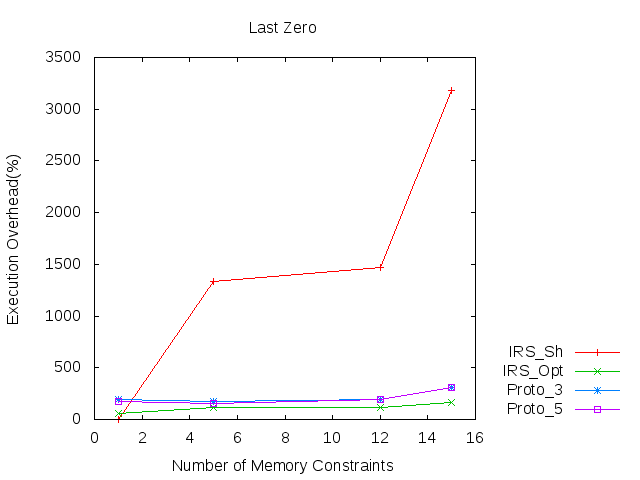
\includegraphics[scale=0.5]{../../evaluations/cores_2/eval_last_zero_best.png}\label{last_zero_best_cores_2}}
     \subfloat[][Comparison between prototypes]{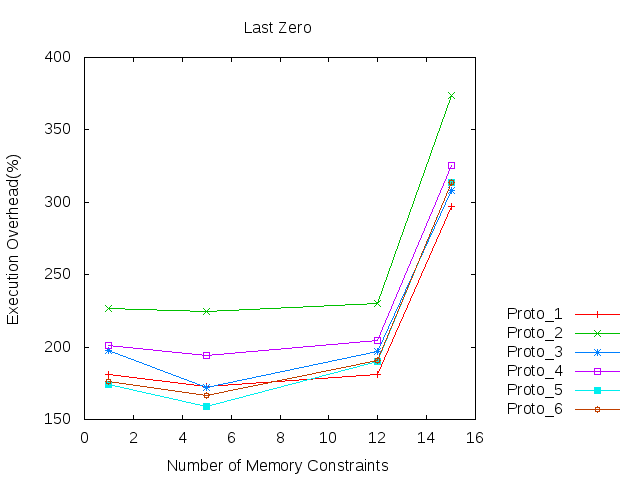
\includegraphics[scale=0.5]
{../../evaluations/cores_2/eval_last_zero_protos.png}
\label{last_zero_protos_cores_2}}
     \caption{Comparison of IRS with Last Zero on two cores}
\end{figure}


\begin{figure}[h]
     \centering
     \subfloat[][User space vs Best Prototype]{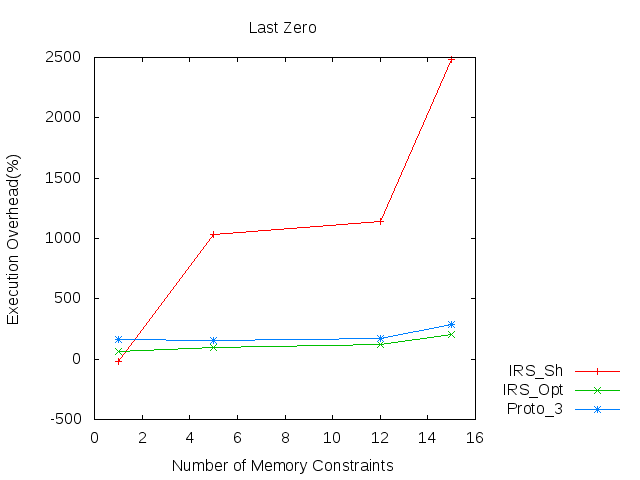
\includegraphics[scale=0.5]{../../evaluations/cores_4/eval_last_zero_best.png}\label{last_zero_best_cores_4}}
     \subfloat[][Comparison between prototypes]{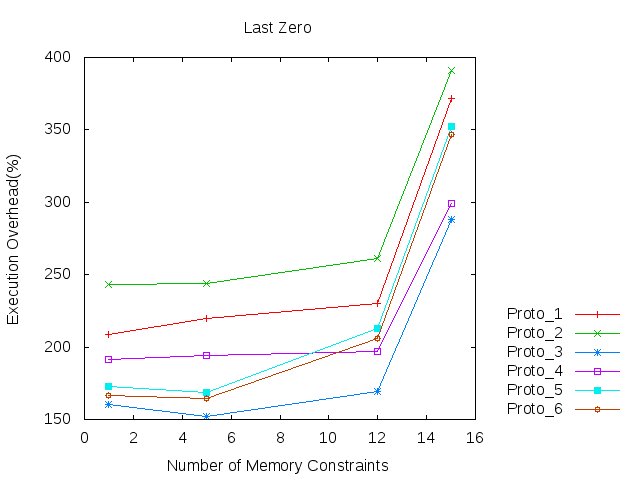
\includegraphics[scale=0.5]{../../evaluations/cores_4/eval_last_zero_protos.png}
\label{last_zero_protos_cores_4}}
     \caption{Comparison of IRS with Last Zero on four cores}
\end{figure}


\begin{figure}[h]
     \centering
     \subfloat[][User space vs Best Prototype]{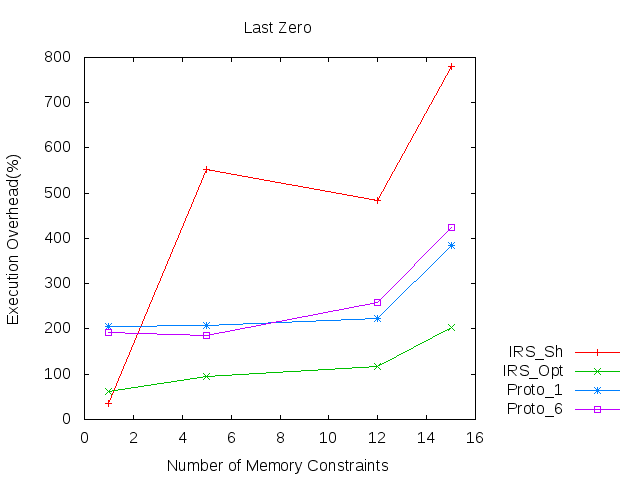
\includegraphics[scale=0.5]{../../evaluations/cores_8/eval_last_zero_best.png}\label{last_zero_best_cores_8}}
     \subfloat[][Comparison between prototypes]{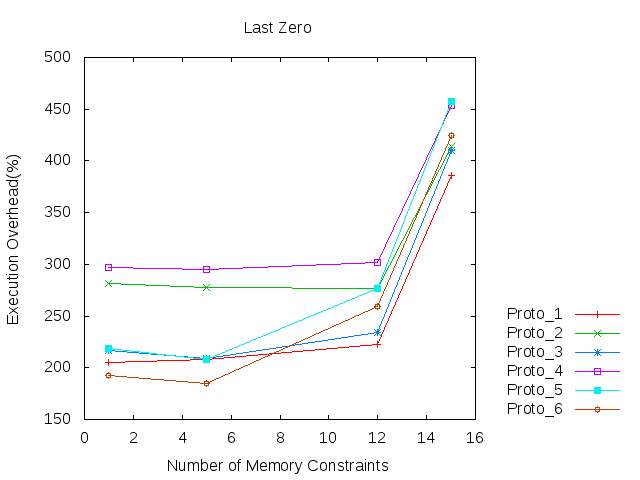
\includegraphics[scale=0.5]{../../evaluations/cores_8/eval_last_zero_protos.png}
\label{last_zero_protos_cores_8}}
     \caption{Comparison of IRS with Last Zero on eight cores}
\end{figure}

This benchmark has 16 threads in total. 
In the first trace file(15 memory constraints), we have atleast one dependency for each thread except for the first thread(thread with id as 0). 
The first trace provides some diversity in the number of memory constraints realized with this benchmark. 
With the evaluation configured for two, four and eight processor cores, we expect the IRS\_Sh to provide the worst performance of the all IRS implementations. 
IRS\_Sh is a busy waiting design. 
Busy waiting design makes the waiting thread to constantly poll one of the cores thus, making it performance inefficient. 
This benchmark has dependencies across all 16 threads with the first trace file and there are more number of threads to the number of processor cores, thus making the busy waiting design to perform poorly among all the other designs for the first trace. 
However, it is expected to improve the execution overhead with the scaling of cores. 
The condition depicted in equation~\ref{mem_cond} satisfies in this benchmark for all the traces thus, making prototypes 5 and 6 to provide the best performance among all the prototypes. 
Section~\ref{fir_app} highlights this condition in more detail manner.  


The results depicted in figures~\ref{last_zero_protos_cores_2}, \ref{last_zero_protos_cores_4}, \ref{last_zero_protos_cores_8} show us that Proto\_1 and Proto\_3 performs better for first trace(number of memory constraints are 15) because the number of memory constraints are closer to the total shared memory events in the benchmarking program. 
From Fig~\ref{last_zero_protos_cores_2}, it is evident that Proto\_5 and Proto\_6 performs nearly the same when it comes to execution overhead. 
For traces which have less number of memory constraints(traces 3, 4 have 5, 1 constraints respectively), Proto\_5 and Proto\_6 performs better among all prototypes in overall. 
From Figures~\ref{last_zero_best_cores_2}, \ref{last_zero_best_cores_4}, \ref{last_zero_best_cores_8}, it is evident that IRS\_Sh performs the worst for this benchmark compared to all the other IRS implementations. 
From Figures~{\ref{last_zero_best_cores_2}, \ref{last_zero_best_cores_4}, \ref{last_zero_best_cores_8}, we observe that execution overhead for IRS\_Sh reduces with the increase in the number of cores. 
From these results, we can extrapolate that the execution overhead would be much lower for IRS\_Sh if the number of processor cores were 16 or more. 
As explained in the previous paragraph, it is because IRS\_Sh is based on a busy waiting design. 
IRS\_Opt provides the best performance among all the IRS solutions under all evaluations of this benchmark. 
It performs better than IRS\_Sh because it uses a condition variable design with an additional thread for handling the scheduling decisions. 
Based on the results for this benchmark, we can conclude that the overhead generated by the pthread library on the IRS\_Opt would be less compared to all the other IRS designs. 
Thus, making IRS\_Opt best choice among all the IRS designs for benchmarks which follow similar conditions and configurations to this benchmark. 




%----------------------------------------------------------------------------
\subsection{Indexer}



%Evaluation of indexer with cores-------
\begin{figure}[h]
     \centering
     \subfloat[][User space vs Best Prototype]{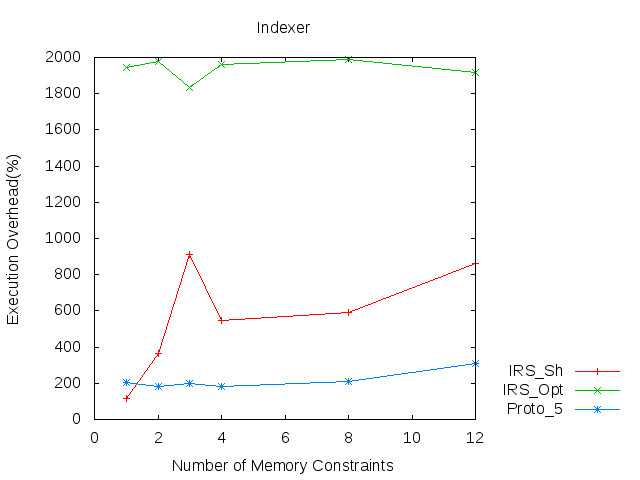
\includegraphics[scale=0.5]{../../evaluations/cores_2/eval_indexer_best.png}\label{indexer_best_cores_2}}
     \subfloat[][Comparison between prototypes]{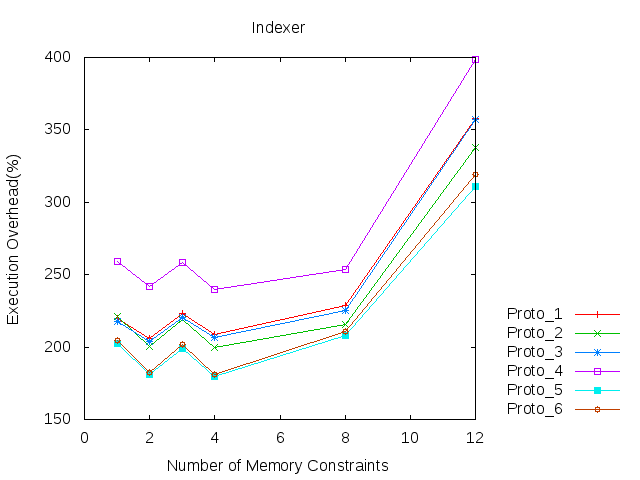
\includegraphics[scale=0.5]{../../evaluations/cores_2/eval_indexer_protos.png}\label{indexer_protos_cores_2}}
     \caption{Comparison of IRS with Indexer on two cores}
\end{figure}


\begin{figure}[h]
     \centering
     \subfloat[][User space vs Best Prototype]{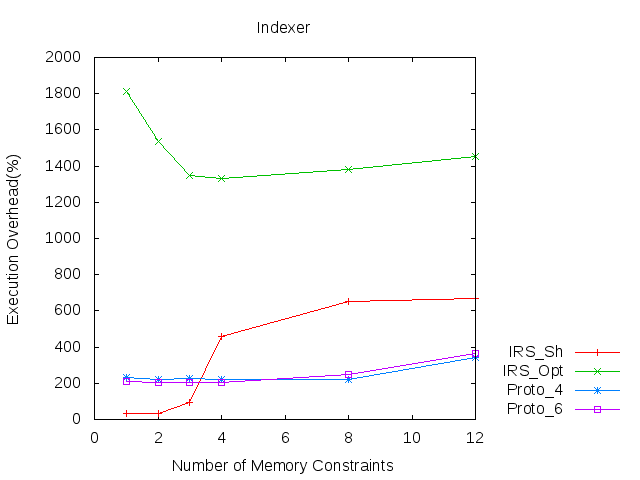
\includegraphics[scale=0.5]{../../evaluations/cores_4/eval_indexer_best.png}\label{indexer_best_cores_4}}
     \subfloat[][Comparison between prototypes]{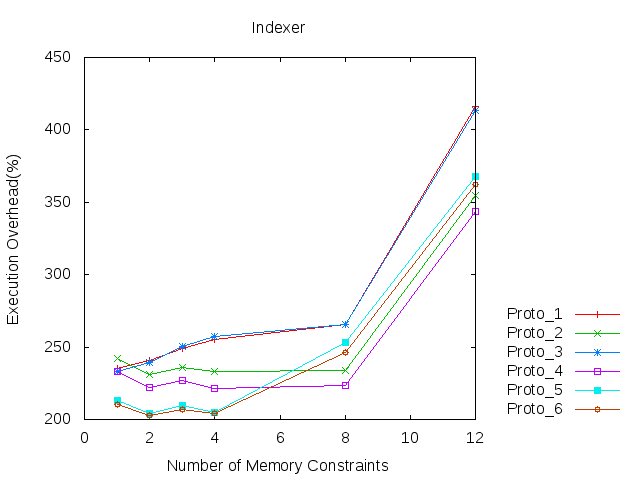
\includegraphics[scale=0.5]{../../evaluations/cores_4/eval_indexer_protos.png}\label{indexer_protos_cores_4}}
     \caption{Comparison of IRS with Indexer on four cores}
\end{figure}


\begin{figure}[h]
     \centering
     \subfloat[][User space vs Best Prototype]{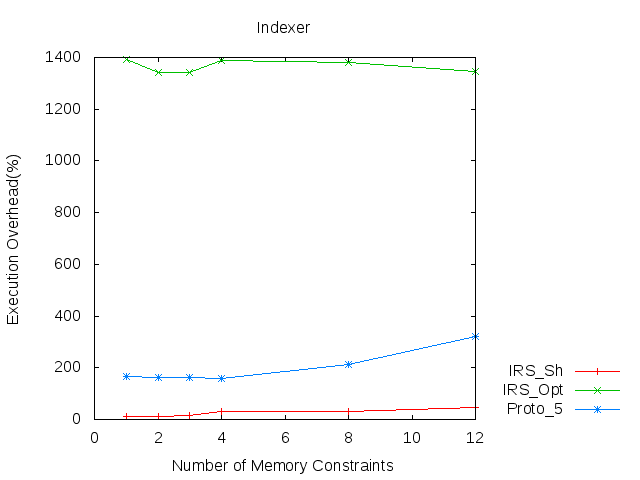
\includegraphics[scale=0.5]{../../evaluations/cores_8/eval_indexer_best.png}\label{indexer_best_cores_8}}
     \subfloat[][Comparison between prototypes]{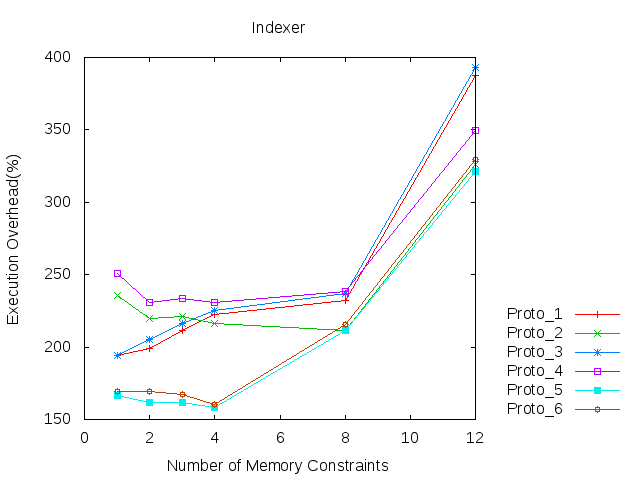
\includegraphics[scale=0.5]{../../evaluations/cores_8/eval_indexer_protos.png}\label{indexer_protos_cores_8}}
     \caption{Comparison of IRS with Indexer on eight cores}
\end{figure}

\citet{dynamic_por} utilize this benchmark for evaluating their dynamic POR design. 
The pseudo code for the indexer program is realized in listing~\ref{code_indexer}.  
The indexer program revolves around a hash table, where threads read and write hashed messages on it. 
Each thread calculates four messages and writes them to a shared hash table. 
Collisions are detected and avoided using the compare and swap(cas) statement. 
The message values depend on the thread id. 

For our experiments, we have used 15 threads with the indexer program. 
The benchmark contains approximately 60 shared-memory events in total. 
Six traces are used with the following as the number of memory constraints: 12, 8, 4, 3, 2, 1. 
The memory constraints are set in a way that all the constraints are within a span of four threads and not all 15 threads. 
For the first trace, we have three memory constraints in each of the four threads.
We expect to have good performance for IRS\_Sh because the number of constraints are not spread across all 15 threads. 
We expect it to perform the best when the core count is 8, even when the number of constraints are set at 12. 
Proto\_5 and Proto\_6 are expected perform best among all the prototypes for this benchmark, because the condition indicated in equation~\ref{mem_cond} satisfies. 

From figures~\ref{indexer_protos_cores_2}, \ref{indexer_protos_cores_4}, \ref{indexer_protos_cores_8}, it is evident that Proto\_5 and Proto\_6 performs the best among the prototypes in all scenarios for this benchmark. 
Based on the analysis of figures~\ref{indexer_best_cores_2}, \ref{indexer_best_cores_4}, \ref{indexer_best_cores_8}\, we observe a trend in the improvement of execution overhead in IRS\_Sh. 
As expected IRS\_Sh provides the best performance when the number of cores is eight as observed in Figure~\ref{indexer_best_cores_8}.
However, IRS\_Opt showcases a huge overhead for this benchmark. 
One of the reasons for such a poor performance would be the lack of diversity of memory constraints(diversity indicates that the memory constraints are within a span of four threads not all 15 threads). 
There are few anomalies in the results, such as the increase in execution overhead for IRS\_Opt when number of memory constraints is 1 as shown in figure~\ref{indexer_best_cores_4}. 
There is no theoretical explanation for such an increase. 
Another anomaly is when the number of memory constraints is 3 and the configuration for processor count is set to two as shown in figures~\ref{indexer_protos_cores_2} and \ref{indexer_best_cores_2}, we observe an increase in execution overhead for all designs except IRS\_Opt. 
The trace file with three memory constraints spans three threads. 
Thus, making a one thread sleep longer in such a scenario eventually creating a surge in execution overhead. 




%----------------------------------------------------------------------------
\subsection{Dining Philosopher's Problem}

%Evaluation of Dining Phil with cores-------
\begin{figure}[h]
     \centering
     \subfloat[][User space vs Best Prototype]{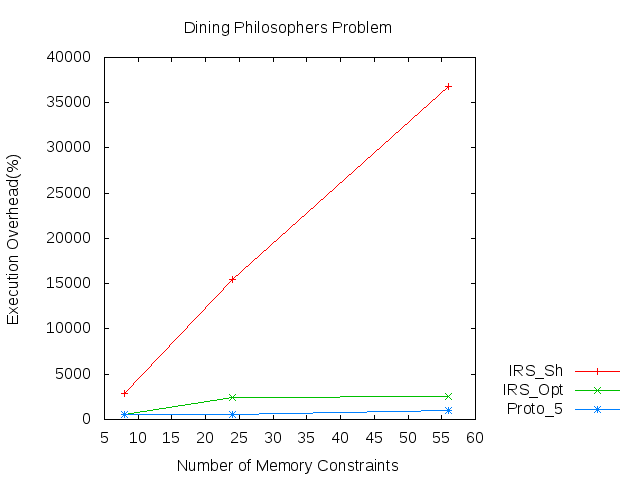
\includegraphics[scale=0.5]{../../evaluations/cores_2/eval_dining_phil_best.png}\label{dining_phil_best_cores_2}}
     \subfloat[][Comparison between prototypes]{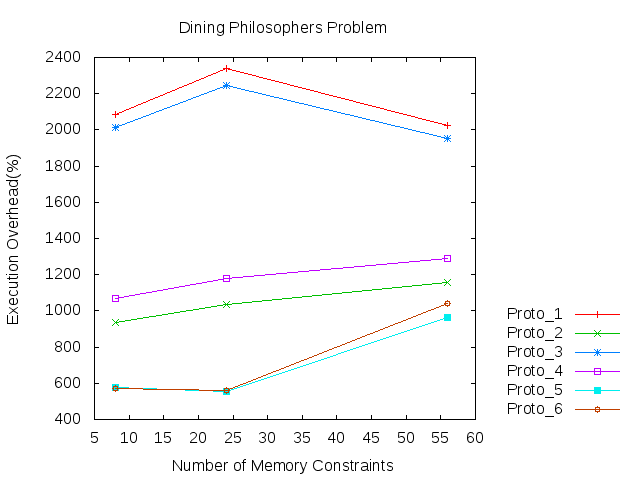
\includegraphics[scale=0.5]{../../evaluations/cores_2/eval_dining_phil_protos.png}\label{dining_phil_protos_cores_2}}
     \caption{Comparison of IRS with Dining Philosophers Problem on two cores}
\end{figure}

\begin{figure}[h]
     \centering
     \subfloat[][User space vs Best Prototype]{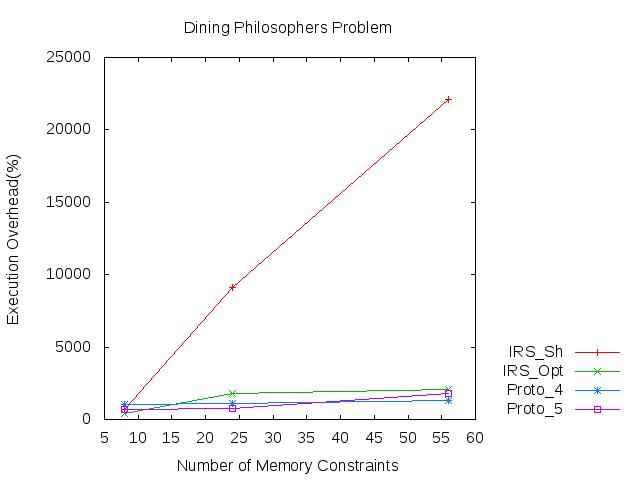
\includegraphics[scale=0.5]{../../evaluations/cores_4/eval_dining_phil_best.png}\label{dining_phil_best_cores_4}}
     \subfloat[][Comparison between prototypes]{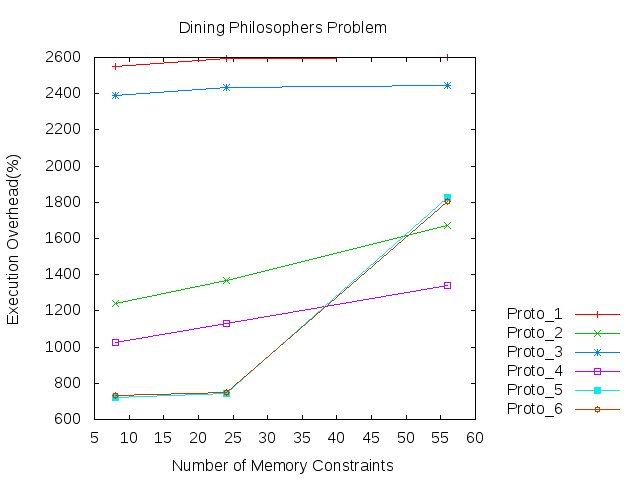
\includegraphics[scale=0.5]{../../evaluations/cores_4/eval_dining_phil_protos.png}\label{dining_phil_protos_cores_4}}
     \caption{Comparison of IRS with Dining Philosophers Problem on four cores}
\end{figure}

\begin{figure}[h]
     \centering
     \subfloat[][User space vs Best Prototype]{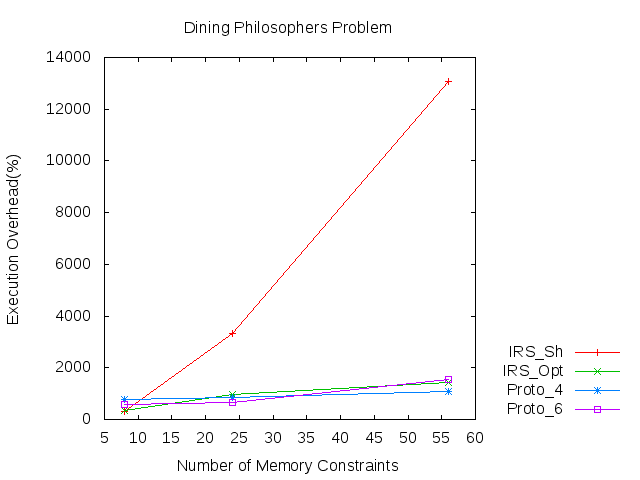
\includegraphics[scale=0.5]{../../evaluations/cores_8/eval_dining_phil_best.png}\label{dining_phil_best_cores_8}}
     \subfloat[][Comparison between prototypes]{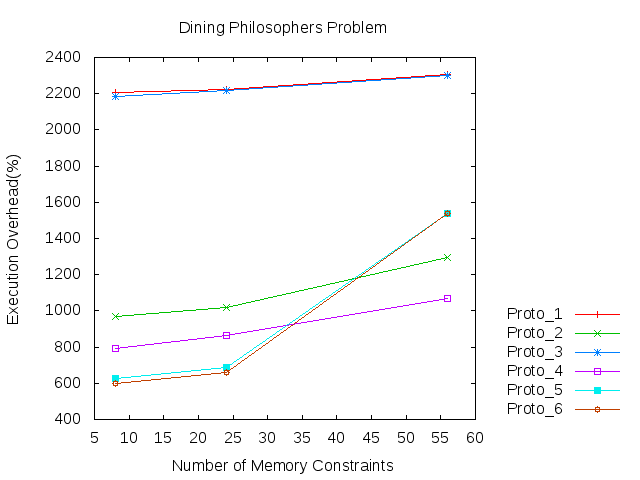
\includegraphics[scale=0.5]{../../evaluations/cores_8/eval_dining_phil_protos.png}\label{dining_phil_protos_cores_8}}
     \caption{Comparison of IRS with Dining Philosophers Problem on eight cores}
\end{figure}

The Dining Philosopher's Problem is a well known synchronization problem in the domain of concurrency problems. 
There are many solutions adhered to overcome the problem. 
\citet{silberschatz2014operating} have addressed many solutions in their book for the above problem. 
We are using one of the solutions proposed in their book. 
The solution uses two classes of philosophers - odd and even philosopher. 
The classification is based on the thread id of the philosopher threads. 
Every odd philosopher checks the chopstick on the left before checking on the right for availability. 
The opposite in case of even philosopher. 
The solution for this problem is showcased in listing~\ref{code_dining_phil}.

In our experiments, we have adapted the solution to have 16 threads and 10 iterations. 
Compared to previous benchmarks which had only few constraints, this benchmark has more constraints and spans across all 16 threads. 
This benchmark is expected to run in milliseconds time range rather than microseconds which was evident with respect to the previous benchmarks. 
For getting a detailed understanding of the experimental results, please refer to appendix~\ref{appendixb}.  

This benchmark has 16 threads at its disposal. 
There are nearly 60 shared-memory events per thread. 
Thus, making a total of 960 shared-memory events in total. 
The benchmark has at-most eight threads running at any point of time. 
The number of memory constraints listed for the three traces include: 56, 24, 8. 
The first trace contains memory constraints spanning all the threads.
This benchmark satisfies the condition depicted in equation~\ref{mem_cond} in all trace file conditions. 
Prototype 1-4 follow the first approach discussed in section~\ref{fir_app}. 
Evaluation on the number of necessary synchronization calls highlighted in section~\ref{vol_kernel_calls}, infers that the prototypes 1-4 to perform poorly when the condition mentioned in equation~\ref{mem_cond} satisfies. 
Among prototypes 1-4, we expect prototype 1 and 3 to perform the worst under these conditions. 
Proto\_1 and Proto\_3 are kernel space solutions implemented with a shared scheduler in place. 
Proto\_1 and Proto\_3, performs $signal\_other\_threads$ call from $AfterMA()$ of every shared memory event. 
As depicted in section~\ref{nocheck}, signaling of other threads is a costly operation compared to updating a vector clock(prototypes 2 and 4 updates vector clock instead of signaling threads). 
Thus, making Proto\_1 and Proto\_3 to perform the worst among the prototypes. 
We expect Proto\_5 and Proto\_6 to provide the best performance among the prototypes because of the condition mentioned in equation~\ref{mem_cond}.
IRS\_Sh is expected to give away a very poor performance because of the diversity of constraints and since it is based on busy waiting design.  

From figures~\ref{dining_phil_protos_cores_2}, \ref{dining_phil_protos_cores_4}, \ref{dining_phil_protos_cores_8}, it is evident that Proto\_5 and Proto\_6 perform the best among the prototypes under all the scenarios of this benchmark. 
Proto\_1 and Proto\_3 as expected came up with the worst performance among the prototypes. 
In case of the comparison with the user space implementation, IRS\_Opt seems to have the smaller overhead compared to IRS\_Sh. 
From Figs~\{\ref{dining_phil_best_cores_2}, \ref{dining_phil_best_cores_4}, \ref{dining_phil_best_cores_8}\}, it is evident that IRS\_Sh seems to have the worst performance for this benchmark because of its busy waiting design. 
However, with the increase in the number for processor cores we can observe a reduction in the execution overhead for IRS\_Sh. 

\subsection{Inference on the scaling of processor cores}

The experiments performed by scaling the processor cores provided valuable insight into the design problems existent in the IRS implementations.  
From the results of benchmarks- Last Zero, Indexer, Dining Philosophers Problem, it is evident that the prototypes do not scale well when the number of cores are increased.
This situation is evident with the first trace(first trace contains the highest number of memory constraints among all the traces for a given benchmark) of each benchmark as depicted in all the results. 
In kernel space for all prototypes, we have implemented vector clocks as a C struct containing an array of integer. 
Such a design was meant to provide good readability and also better memory referencing when invoked from different function. 
However, such a design drastically suffers from the problem of false sharing. 
For getting a better understanding of false sharing please refer to appendix~\ref{appendixc}.
Such an impact is clearly evident with the scaling of processor cores on the results of all three benchmarks.

\section{Inference}

The Fibonacci benchmark helped us in understanding the behavior of prototypes. 
The experiments by scaling the processor cores clearly explained the merits and demerits of various IRS designs. 
All the experiments show that Proto\_5 and Proto\_6 seem to perform the best among the prototypes in nearly all the scenarios given in the bench-marking programs. 
IRS\_Sh implementation seems to give away the worst performance in nearly all benchmarks. 
From the experiments, it is evident that all prototypes suffer from the problem of scalability. 
The IRS user space implementations performs better than the IRS kernel space implementations, when the number of memory constraints are in single digits and the number of memory constraints are comparably large. 
 
By observing the above results we can conclude that there is a need of a solution which is the combination of IRS\_Opt and Prototypes 5-6. 
This implementation would have a loadable kernel module similar to Proto\_5 or Proto\_6 however, without any checking for memory permissions in kernel space for the threads. 
The kernel module would help in providing as a forced yield of the processor to the OS Scheduler from the thread and also an interface to revive the thread. 
The check for memory access permission would be implemented entirely in the user space and calls would be made to the above mentioned kernel space solution for yielding the processor.  
In short, this kernel space interface would be used instead of using condition variables in IRS\_Opt.
